
\section*{Proof of homotopy}

\begin{theorem}
Let $(A,V, i,p,h)$ be a deformation retraction, where $A$ is a DG-algebra and $V$ is a chain complex. Let $m_2$ be the induced transferred product on $V$. Then the operation $m_3$, as described in \ref{sec:deformation_retraction}, is a homotopy between $m_2(id\otimes m_2)$ and $m_2(m_2\otimes id)$. 
\end{theorem}

We have not come upon a fully written out detailed proof, so to have at least one existing complete calculation in the world, we have maybe been overly thorough. It is not pretty, and it is just tedious straight forward calculation, but in our opinion it is nice to have, as it gives some insight into how these homotopies between operations work. 

We denote $d_A$ by just $d$, and $id$ by $1$ in order to make it more distinguishable from $d$ and eventual copies of $i\circ d$. We also skip writing $\circ$, and denote it instead just by concatenation, so $d\circ m_3 = dm_3$. Since $m_3$ consists of $i, p$, which are both of degree $0$, and $h$, which has degree $-1$, we have $|m_3|=-1$. The boundary of $m_3$ is then
\begin{align*}
    \partial m_3 
    &= dm_3+m_3(d,1,1)+m_3(1,d,1)+m_3(1,1,d)\\
    &= dm_3
    +p((-1)^{|1||d|}m(hm(id\otimes i)\otimes i)
    -(-1)^{|hm||d|}m(id\otimes hm(i\otimes i))) \\
    & \hspace{13mm} 
    +p((-1)^{|1||1|}m(hm(i\otimes id)\otimes i)
    -(-1)^{|hm||1|}m(i\otimes hm(id\otimes i))) \\
    & \hspace{13mm} 
    +p((-1)^{|1||1|}m(hm(i\otimes i)\otimes id)
    -(-1)^{|hm||1|}m(i\otimes hm(i\otimes id)))
\end{align*}

where the signs appear due to the Koszul grading rule\index{The Koszul grading rule}. As the identity morphism has degree $0$ most of these vanish, except for $(-1)^{|hm||d|}$. The composite map $hm$ has degree $|h|+|m| = -1+0 = -1$ and the differential $d$ has degree $1$ as we work with cohomological grading. Since $i$ is a morphism of chain complexes it commutes with the differentials, hence we can put all the $i$'s to the right, to get 
\begin{align*}
    \partial m_3 
    &= dm_3
    +p(m(hm(d\otimes 1)\otimes 1)
    +m(d\otimes hm) \\
    & \hspace{17mm} 
    +m(hm(1\otimes d)\otimes 1)
    -m(1\otimes hm(d\otimes 1)) \\
    & \hspace{17mm} 
    +m(hm\otimes d)
    -m(1\otimes hm(1\otimes d))(i\otimes i\otimes i)
\end{align*}

We haven't touched the $dm_3$ part yet, so lets see what this gives us. We get 
\begin{align*}
    dm_3 
    &= 
    d(p(m(hm\otimes 1)
    -m(1\otimes hm))(i\otimes i\otimes i)) \\
    &= 
    p(dm(hm\otimes 1)
    -dm(1\otimes hm))(i\otimes i\otimes i) \\
\end{align*}

Since $A$ is a DG-algebra we can use the graded Leibniz rule\index{The Leibniz rule} to expand $dm$ into $m(d\otimes 1)+m(1\otimes d)$. Doing so both places they appear above gives us
\begin{align*}
    dm_3 
    &= 
    p((m(d\otimes 1)
    +m(1\otimes d))(hm\otimes 1) \\
    &\quad 
    -(m(d\otimes 1)
    +m(1\otimes d))(1\otimes hm))(i\otimes i\otimes i) \\
    &=
    p((m(d\otimes 1)
    +m(1\otimes d))(hm\otimes 1) \\
    &\quad 
    -m(d\otimes 1)
    -m(1\otimes d)(1\otimes hm))(i\otimes i\otimes i) 
\end{align*}

To contract this we again need to apply the Koszul grading rule. For the individual pieces in the above equation we get
\begin{align*}
    m(d\otimes 1)(hm\otimes 1) &= (-1)^{|1||hm|}m(dhm\otimes 1) \\
    m(1\otimes d)(hm\otimes 1) &= (-1)^{|d||hm|}m(hm\otimes d) \\
    m(d\otimes 1)(1\otimes hm) &= (-1)^{|1||1|}m(d\otimes hm) \\
    m(1\otimes d)(1\otimes hm) &= (-1)^{|d||1|}m(1\otimes dhm),
\end{align*}

where as before all signs are $1$ except $(-1)^{|d||hm|}=-1$. Hence we have 
\begin{align*}
    dm_3 
    &= 
    p(m(dhm\otimes 1)-m(hm\otimes d)-m(d\otimes hm)-m(1\otimes dhm))(i\otimes i\otimes i)
\end{align*}

We know that $h$ is a homotopy\index{Homotopy of chain maps} between $i\circ p$ and $id_A$, and for chain complexes this means that $dh+hd=i\circ p - id_A$. This gives us that we can replace $dh$ by $id_A-i\circ p-hd$ in the equation above. Doing this gives us 
\begin{align*}
    dm_3 
    &= 
    p(m((1-ip-hd)m\otimes 1)-m(hm\otimes d)-m(d\otimes hm) \\
    &\quad -m(1\otimes (1-ip-hd)m))(i\otimes i\otimes i) \\
    &= 
    p(m(m\otimes 1)-m(ipm\otimes 1)-m(hdm\otimes 1) \\
    &\quad -m(hm\otimes d)-m(d\otimes hm) \\
    &\quad -m(1\otimes m)+m(1\otimes ipm)+m(1\otimes hdm))(i\otimes i\otimes i)
\end{align*}

Notice that we have both $m(m\otimes 1)$ and $m(1\otimes m)$ present, with the opposite signs. These two are just repeated products in $A$, so their difference is $0$, as we know $A$ is a DG-algebra, which in particular have an associative product.

After canceling the associator in $A$, and rearranging the terms a bit nicer, we can venture further by again applying the graded Leibniz rule to the $dm$'s. This gives us
\begin{align*}
    dm_3 
    &=
    p(m(1\otimes ipm)-m(ipm\otimes 1) \\
    &\quad -m(h(m(d\otimes 1)+m(1\otimes d))\otimes 1) \\
    &\quad -m(hm\otimes d)-m(d\otimes hm) \\
    &\quad +m(1\otimes h(m(d\otimes 1)+m(1\otimes d))))(i\otimes i\otimes i) \\
    &=
    p(m(1\otimes ipm)-m(ipm\otimes 1) \\
    &\quad - m(hm(d\otimes 1)\otimes 1) - m(hm(1\otimes d)\otimes 1) \\
    &\quad +m(hm\otimes d)+m(d\otimes hm) \\
    &\quad +m(1\otimes hm(d\otimes 1))+m(1\otimes hm(1\otimes d)))(i\otimes i\otimes i)
\end{align*}

Now we are finally ready to put everything together. Recall we wanted to find $\partial m_3 = dm_3 + m_3d_{A^{\otimes 3}}$. The calculation has been so long that it is hard to remember what we actually were doing. We have found both parts of this equation, so putting them together and moving all the $p$'s to the left, and the $i$'s to the right, we get
\begin{align*}
    \partial m_3
    &=
%    p(m(1\otimes ipm)-m(ipm\otimes 1) \\
%    &\quad - m(hm(d\otimes 1)\otimes 1) - m(hm(1\otimes d)\otimes 1) \\
%    &\quad -m(hm\otimes d)-m(d\otimes hm) \\
%    &\quad +m(1\otimes hm(d\otimes 1))+m(1\otimes hm(1\otimes d))(i\otimes i\otimes i) \\
%    &\quad
%    +p(m(hm(d\otimes 1)\otimes 1)
%    +m(d\otimes hm) \\
%    &\quad 
%    +m(hm(1\otimes d)\otimes 1)
%    -m(1\otimes hm(d\otimes 1)) \\
%    &\quad  
%    +m(hm\otimes d)
%    -m(1\otimes hm(1\otimes d))(i\otimes i\otimes i) \\
%    &= 
    p(m(1\otimes ipm)-m(ipm\otimes 1) \\
    &\quad - m(hm(d\otimes 1)\otimes 1) - m(hm(1\otimes d)\otimes 1) \\
    &\quad -m(hm\otimes d)-m(d\otimes hm) \\
    &\quad +m(1\otimes hm(d\otimes 1))+m(1\otimes hm(1\otimes d) \\
    &\quad
    +m(hm(d\otimes 1)\otimes 1)
    +m(d\otimes hm) \\
    &\quad 
    +m(hm(1\otimes d)\otimes 1)
    -m(1\otimes hm(d\otimes 1)) \\
    &\quad  
    +m(hm\otimes d)
    -m(1\otimes hm(1\otimes d))(i\otimes i\otimes i)
\end{align*}
%where in the last equality we have just put the $p$ on the left and the $i$'s on the right. This is just to have everything inside the same bracket, i.e. $p(\text{all the stuff})(i\otimes i\otimes i)$, which we can do as they are linear. 
We see that almost everything on the inside cancels nicely, and we are left with 
\begin{equation*}
    \partial m_3 = p(m(1\otimes ipm)-m(ipm\otimes 1))(i\otimes i\otimes i)
\end{equation*}

Expanding this we get 
\begin{equation*}
    \partial m_3 = pm(1\otimes ipm)(i\otimes i\otimes i) - pm(ipm\otimes 1)(i\otimes i\otimes i)
\end{equation*}

which we recognize as $m_2(1\otimes m_2) - m_2(m_2\otimes 1)$. This means we are finally left with what we wanted to show 
\begin{equation*}
    \partial m_3 = m_2(1\otimes m_2)-m_2(m_2\otimes 1)
\end{equation*}
i.e. the associator of $m_2$. 

As $m_3$ is a homotopy of the associator, we call it the associating homotopy\index{Associating homotopy}.


\section*{Proof of deformation retraction}

Let $A=(\bigoplus_{i\in \Z}A^i, d, m)$ be a DG-algebra. As usual we denote $Z^n = \ker d^n$, the $n$-cochains,  and $B^n = \ima d^{n-1}$, the $n$-coboundaries. Since $A$ is in particular a cochain complex we know that $B^n\subseteq Z^n$ is a subspace, i.e. all coboundaries are cocycles. This means that we can find a subspace $H^n$ of $Z^n$ such that $Z^n = B^n\oplus H^n$. Notice that we can identify $H^n(A)\cong H^n$ as we have a split exact sequence
\begin{equation*}
    0\longrightarrow B^n\longrightarrow Z^n\overset{d^n}\longrightarrow H^n(A)\longrightarrow 0 .
\end{equation*}
As $Z^n$ is a subspace of $A^n$ we can also find another subspace $L^n$ such that 
\begin{equation*}
    A^n = Z^n\oplus L^n = B^n\oplus H^n\oplus L^n
\end{equation*}
We can identify $L^n$ with $B^{n+1}$ because of the existence of the split exact sequence 
\begin{equation*}
    0\longrightarrow Z^n\longrightarrow A^n\overset{d^n}\longrightarrow B^{n+1}\longrightarrow 0
\end{equation*}

We can also view the cohomology algebra $H(A)$ as a sub algebra through the identification with $H=\bigoplus_{i\in \Z} H^n$. Denote $i\colon H\longrightarrow A$ the inclusion of $H$ into $A$ and $p\colon A\longrightarrow H$ the projection. Notice that we have $p\circ i = id_H$. The only remaining part---in order to have a deformation retraction---is the homotopy $h\colon A\longrightarrow A$. We will chose this homotopy quite carefully. 

Let us first define some notation. Since $A^n=B^n\oplus H^n\oplus L^n$ we can describe the differential $d$ by nine maps 
\begin{alignat*}{3}
    d^n_{BB}&\colon B^n &&\longrightarrow B^{n+1} \\
    d^n_{BH}&\colon B^n &&\longrightarrow H^{n+1} \\
    d^n_{BL}&\colon B^n &&\longrightarrow L^{n+1} \\
    d^n_{HB}&\colon H^n &&\longrightarrow B^{n+1} \\
    d^n_{HH}&\colon H^n &&\longrightarrow H^{n+1} \\
    d^n_{HL}&\colon H^n &&\longrightarrow L^{n+1} \\
    d^n_{LB}&\colon L^n &&\longrightarrow B^{n+1} \\
    d^n_{LH}&\colon L^n &&\longrightarrow H^{n+1} \\
    d^n_{LL}&\colon L^n &&\longrightarrow L^{n+1} , 
\end{alignat*}
each of them being just the differential projected and restricted to the proper part of the decomposition of $A$. Equivalently they are the parts of the matrix describing the differential, i.e. 
\begin{equation*}
d^n = 
\begin{bmatrix}
    d^n_{BB} & d^n_{BH} & d^n_{BL} \\
    d^n_{HB} & d^n_{HH} & d^n_{HL} \\
    d^n_{LB} & d^n_{LH} & d^n_{LL} 
\end{bmatrix}
\colon B^n\oplus H^n\oplus L^n \longrightarrow B^{n+1}\oplus H^{n+1}\oplus L^{n+1}
\end{equation*}
Because $B^n$ and $H^n$ both consist of cocycles, we know that the differential vanishes on those subspaces. Hence we have 
\begin{equation*}
    d^n_{BB} = d^n_{BH} = d^n_{BL} = d^n_{HB} = d^n_{HH} = d^n_{HL} = 0.
\end{equation*}
We also have no $(n+1)$-coboundaries in $H^{n+1}$ and $L^{n+1}\cong B^{n+2}$, which means we have $d^n_{LH} = d^n_{LL} = 0$ as well.

This means that the matrix for $d^n$ really looks like
\begin{equation*}
d^n = 
\begin{bmatrix}
    0 & 0 & 0 \\
    0 & 0 & 0 \\
    d^n_{LB} & 0 & 0 
\end{bmatrix}    
\end{equation*}

We can now describe the degree $n$ part of our proposed homotopy $h$ as a map 
\begin{equation*}
    h^n\colon B^n\oplus H^n\oplus L^n \longrightarrow B^{n-1}\oplus H^{n-1}\oplus L^{n-1} 
\end{equation*}
given by the matrix 
\begin{equation*}
h^n = 
\begin{bmatrix}
0 & 0 & (d_{LB}^{n-1})^{-1}\\
0 & 0 & 0\\
0 & 0 & 0
\end{bmatrix}
\end{equation*}
Note that this inverse, $(d_{LB}^{n-1})^{-1}$, exists, as we earlier identified the subspace $L^n$ by $L^n \cong B^{n+1}$. 

In order for $h$ to be a homotopy between $id_A$ and $i\circ p$, we need to have 
\begin{equation*}
    id_{A^n} - (i\circ p)^n = d^{n-1}\circ h^{n} + h^{n+1}\circ d^n, 
\end{equation*}
or equivalently stated---that the sum of the maps in the parallelogram in the below diagram, equals the vertical arrow. 
\begin{center}
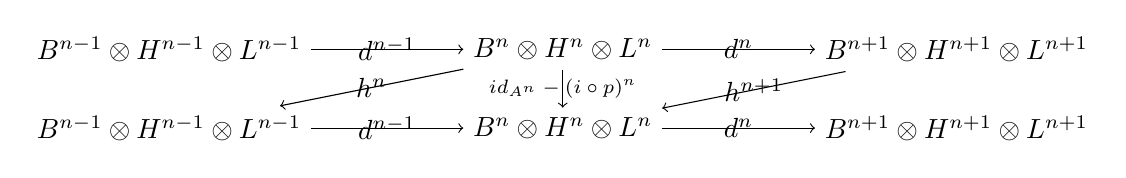
\begin{tikzpicture}
	\node (1) {$B^{n-1}\otimes H^{n-1}\otimes L^{n-1}$};
	\node (2) [node distance=5cm, right of=1] {$B^n\otimes H^n\otimes L^n$};
	\node (3) [node distance=5cm, right of=2] {$B^{n+1}\otimes H^{n+1}\otimes L^{n+1}$};
	
	\node (4) [below of=1]{$B^{n-1}\otimes H^{n-1}\otimes L^{n-1}$};
	\node (5) [node distance=5cm, right of=4] {$B^n\otimes H^n\otimes L^n$};
	\node (6) [node distance=5cm, right of=5] {$B^{n+1}\otimes H^{n+1}\otimes L^{n+1}$};

	\draw [-to] (2) to node [swap]{$h^n$} (4);
	\draw [-to] (3) to node {$h^{n+1}$} (5);
	\draw [-to] (2) to node {{\scriptsize $id_{A^n}-(i\circ p)^n$}} (5);
	
	\draw [-to] (1) to node {$d^{n-1}$} (2);
	\draw [-to] (2) to node {$d^{n}$} (3);
	\draw [-to] (4) to node [swap]{$d^{n-1}$} (5);
	\draw [-to] (5) to node [swap]{$d^{n}$} (6);
\end{tikzpicture}
\end{center}

In matrix notation the left hand side becomes
\begin{equation*}
\begin{bmatrix}
1 & 0 & 0 \\
0 & 1 & 0 \\
0 & 0 & 1
\end{bmatrix}
-
\begin{bmatrix}
0 & 0 & 0 \\
0 & 1 & 0 \\
0 & 0 & 0
\end{bmatrix}
=
\begin{bmatrix}
1 & 0 & 0 \\
0 & 0 & 0 \\
0 & 0 & 1
\end{bmatrix}
\end{equation*}
so we need to confirm that the right hand side is equal to that. We just multiply the matrices we have for the maps, which gives us
\begin{align*}
    d^{n-1}\circ h^n 
    &= 
    \begin{bmatrix}
    0 & 0 & 0 \\
    0 & 0 & 0 \\
    d^{n-1}_{LB} & 0 & 0
    \end{bmatrix}
    \cdot
    \begin{bmatrix}
    0 & 0 & (d_{LB}^{n-1})^{-1}\\
    0 & 0 & 0\\
    0 & 0 & 0
    \end{bmatrix} \\
    &= 
    \begin{bmatrix}
    0 & 0 & 0 \\
    0 & 0 & 0 \\
    0 & 0 & d^{n-1}_{LB}(d_{LB}^{n-1})^{-1} 
    \end{bmatrix} \\
    &= 
    \begin{bmatrix}
    0 & 0 & 0 \\
    0 & 0 & 0 \\
    0 & 0 & 1 
    \end{bmatrix}
\end{align*}
and
\begin{align*}
    h^{n+1}\circ d^n 
    &=
    \begin{bmatrix}
    0 & 0 & (d_{LB}^{n})^{-1}\\
    0 & 0 & 0\\
    0 & 0 & 0
    \end{bmatrix}
    \cdot 
    \begin{bmatrix}
    0 & 0 & 0 \\
    0 & 0 & 0 \\
    d^{n}_{LB} & 0 & 0
    \end{bmatrix} \\
    &=
    \begin{bmatrix}
    (d_{LB}^{n})^{-1}d^{n}_{LB} & 0 & 0\\
    0 & 0 & 0\\
    0 & 0 & 0
    \end{bmatrix} \\
    &=
    \begin{bmatrix}
    1 & 0 & 0\\
    0 & 0 & 0\\
    0 & 0 & 0
    \end{bmatrix} .
\end{align*}
Hence we have
\begin{align*}
    h^{n+1}\circ d^n + d^{n-1}\circ h^n 
    &= 
    \begin{bmatrix}
    0 & 0 & 0 \\
    0 & 0 & 0 \\
    0 & 0 & 1 
    \end{bmatrix}
    + 
    \begin{bmatrix}
    1 & 0 & 0 \\
    0 & 0 & 0 \\
    0 & 0 & 0 
    \end{bmatrix} \\
    &= 
    \begin{bmatrix}
    1 & 0 & 0 \\
    0 & 0 & 0 \\
    0 & 0 & 1
    \end{bmatrix} \\
    &= 
    id_{A^n} - (i\circ p)^n , 
\end{align*}
which shows that $h$ is in fact a chain homotopy between $id_A$ and $i\circ p$. This means that we finally have our deformation retraction\index{Deformation retraction}.
\begin{center}
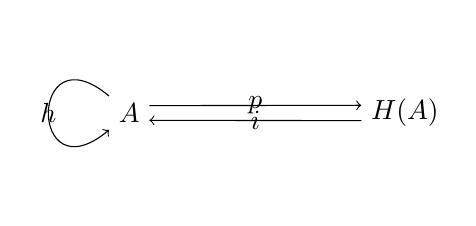
\begin{tikzpicture}
	\node (1) {$A$};
	\node (2) [node distance=3.5cm, right of=1] {$H(A)$};
	
	\draw [to-, out=220, in=140, loop] (1) to node {$h$} (1);
	\draw [-to] (1.20) to node {$p$} (2.170);
	\draw [-to] (2.190) to node {$i$} (1.340); . 
\end{tikzpicture}
\end{center}